\section{Markov不等式}
\label{sec:tail-markov}

回到响应时间。设$X\geq0$，平均$\mathbb{E}[X]=2$秒。有没有可能一半的请求都超过$5$秒？不可能：这一半请求单是自己就给平均值贡献了至少$0.5\times5=2.5$秒，已经超过$2$。这个“远处的质量至少按阈值计入平均”的想法，就是本节的全部内容。

\paragraph{重心的论证}
把分布看成数轴上总量为一的质量，期望是它的重心。质量全在$[0,\infty)$上时，落在$t$右边的那部分质量对重心的贡献至少是“质量乘$t$”；其余质量的贡献至少是$0$。重心又只有$\mathbb{E}[X]$那么远，所以远处的质量不能太多。

\begin{theorem}[Markov不等式]
\label{thm:tail-markov}
设随机变量$X\geq0$，$\mathbb{E}[X]<\infty$。则对每个$t>0$，
\begin{equation}
 \mathbb{P}(X\geq t)\leq\frac{\mathbb{E}[X]}{t} .
 \label{eq:tail-markov}
\end{equation}
\end{theorem}

这个结论称为\term{Markov不等式}（Markov inequality）。证明把“至少贡献$t$”写成两个随机变量之间的比较。

\begin{proof}
考虑示性变量$\mathbf{1}_{\{X\geq t\}}$，它在$X\geq t$时取$1$，否则取$0$。逐个样本点比较$t\,\mathbf{1}_{\{X\geq t\}}$与$X$：若$X\geq t$，左边是$t$，不超过$X$；若$X<t$，左边是$0$，由$X\geq0$也不超过$X$。所以
\[
 t\,\mathbf{1}_{\{X\geq t\}}\leq X .
\]
两边取期望。由期望的保序性和线性性（第~\ref{chap:random-variable-moments}章），以及示性变量的期望就是事件的概率，得到
\[
 t\,\mathbb{P}(X\geq t)\leq\mathbb{E}[X] .
\]
除以$t>0$即得式~\eqref{eq:tail-markov}。
\end{proof}

证明的关键一步是用一个函数从上方压住尾事件的示性函数。图~\ref{fig:tail-dominating}(a)画的就是这一点：蓝色台阶是$\mathbf{1}_{\{x\geq t\}}$，紫色直线是$x/t$，在$x\geq0$上直线处处不低于台阶。取期望后，台阶给出概率，直线给出$\mathbb{E}[X]/t$。另外两个子图是后两节要用的压法，换一个压住台阶的函数，就换一个不等式。

\begin{BookInlineFigure}
 \centering
 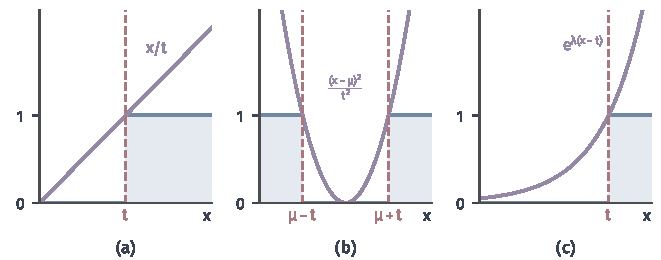
\includegraphics[width=112mm]{figures/07-probability/01-elementary-probability/matplotlib/tail-dominating/figure.pdf}
 \caption{用函数从上方压住尾事件的示性函数。蓝色台阶与浅蓝区域是示性函数，紫线是压住它的函数，红色虚线是阈值。(a)$x\geq0$上的$x/t$。(b)$(x-\mu)^2/t^2$。(c)$\mathrm{e}^{\lambda(x-t)}$，$\lambda>0$。}
 \label{fig:tail-dominating}
\end{BookInlineFigure}

\paragraph{搬动质量的图景}
同一个证明还可以看成搬动质量。把$[0,t)$里的质量全部搬到$0$，把$[t,\infty)$里的质量全部搬到$t$。每块质量只向左移动，重心只会左移；搬完以后，$t$处的质量仍是$\mathbb{P}(X\geq t)$，新重心是$t\,\mathbb{P}(X\geq t)$。于是新重心不超过原重心，这正是$t\,\mathbb{P}(X\geq t)\leq\mathbb{E}[X]$。

图~\ref{fig:tail-markov-mass}用一个六点分布演示。上排质量依次为$0.15$、$0.25$、$0.20$、$0.15$、$0.15$、$0.10$，位于$1$、$2$、$3$、$4$、$6$、$8$，重心为
\[
 \mu=0.15+0.5+0.6+0.6+0.9+0.8=3.55 .
\]
取$t=5$，右边有质量$0.25$。搬动后下排只剩$0$处的$0.75$和$5$处的$0.25$，重心变为$5\times0.25=1.25\leq3.55$。

\begin{BookInlineFigure}
 \centering
 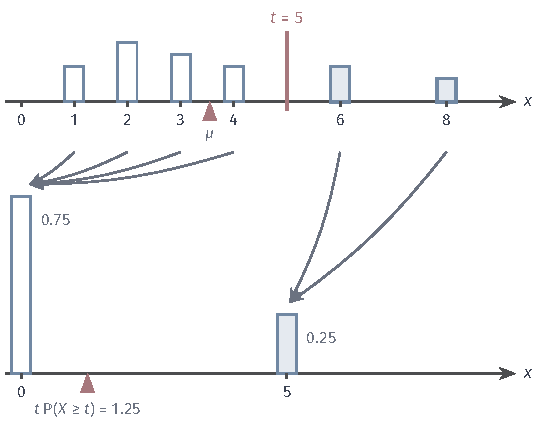
\includegraphics[width=92mm]{figures/07-probability/01-elementary-probability/tikz/tail-markov-mass/figure.pdf}
 \caption{Markov不等式的搬动质量论证。上排是原分布，浅蓝柱是$\{X\geq5\}$的质量，红线是阈值$t=5$，红三角是重心$\mu=3.55$。灰色箭头把$t$左边的质量搬到$0$，把右边的质量搬到$t$。下排是搬动后的两点分布，重心降为$t\,\mathbb{P}(X\geq t)=1.25$。}
 \label{fig:tail-markov-mass}
\end{BookInlineFigure}

\paragraph{面积的图景}
第三种看法用尾积分公式。由式~\eqref{eq:tail-integral-moments}，$\mathbb{E}[X]$是生存函数$s\mapsto\mathbb{P}(X>s)$下方的面积。对$0\leq s<t$，有$\{X\geq t\}\subseteq\{X>s\}$，所以生存函数在$[0,t)$上不低于$\mathbb{P}(X\geq t)$。宽为$t$、高为$\mathbb{P}(X\geq t)$的矩形整个落在曲线下方，面积不超过总面积。

图~\ref{fig:tail-layer-cake}取$X\sim\operatorname{Exp}(1)$与$t=2$。曲线下总面积是$\mu=1$，黄色矩形面积是$2\mathrm{e}^{-2}\approx0.271$。矩形之外的面积就是Markov不等式没有用上的部分：$t$左边曲线高出矩形的那一块，以及$t$右边的整个尾巴。

\begin{BookInlineFigure}
 \centering
 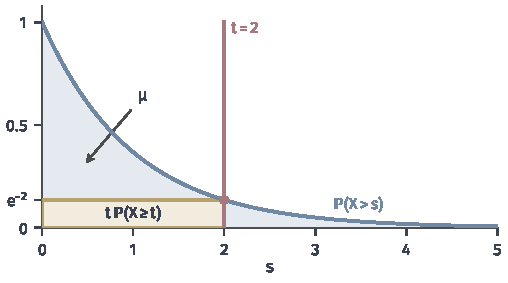
\includegraphics[width=86mm]{figures/07-probability/01-elementary-probability/matplotlib/tail-layer-cake/figure.pdf}
 \caption{$X\sim\operatorname{Exp}(1)$的生存函数（蓝线）。浅蓝区域面积等于$\mu=\mathbb{E}[X]=1$；黄色矩形宽$t=2$、高$\mathbb{P}(X\geq2)=\mathrm{e}^{-2}$，落在曲线下方，所以$t\,\mathbb{P}(X\geq t)\leq\mu$。}
 \label{fig:tail-layer-cake}
\end{BookInlineFigure}

\paragraph{条件的作用}
定理有三个条件，每一个都不能随便去掉。

第一是$X\geq0$。若允许负值，正负质量可以互相抵消，均值不再约束远处的质量。设$X$以各$1/2$的概率取$-100$和$100$，则$\mathbb{E}[X]=0$，但$\mathbb{P}(X\geq1)=1/2$，而式~\eqref{eq:tail-markov}的右边是$0$。证明中失效的一步正是$X<t$时“$0\leq X$”。

第二是$\mathbb{E}[X]<\infty$。若期望为$+\infty$，不等式右边是$+\infty$，仍然成立但不提供任何信息。第三是$t>0$：$t\leq0$时$\{X\geq t\}$是必然事件，概率为$1$，也无需估计。

\paragraph{这个界不能再改进}
Markov不等式只用到均值。它会不会只是证明粗糙，换一种论证就能更紧？答案是否定的：在“非负、均值为$\mu$”这一信息下，它已经是最好的保证。

\begin{theorem}[Markov界的最优性]
\label{thm:tail-markov-sharp}
设$\mu>0$，$t>0$。在所有满足$X\geq0$、$\mathbb{E}[X]=\mu$的随机变量中，$\mathbb{P}(X\geq t)$的最大值为
\begin{equation}
 \sup\,\mathbb{P}(X\geq t)=\min\Bigl\{1,\frac{\mu}{t}\Bigr\} .
 \label{eq:tail-markov-sharp}
\end{equation}
\end{theorem}

\begin{proof}
由Markov不等式和概率不超过$1$，每个这样的$X$都满足$\mathbb{P}(X\geq t)\leq\min\{1,\mu/t\}$。只需构造达到它的分布。

若$\mu\leq t$，令$X$以概率$\mu/t$取$t$，以概率$1-\mu/t$取$0$。它非负，均值为$t\cdot\mu/t=\mu$，并且$\mathbb{P}(X\geq t)=\mu/t$。

若$\mu>t$，令$X$恒等于$\mu$。它的均值是$\mu$，并且$\mathbb{P}(X\geq t)=1$。
\end{proof}

两点分布正是搬动质量后的形状：质量只放在$0$和$t$两处，没有一点“浪费”在比$t$更远的地方，也没有放在$0$与$t$之间。任何具体分布只要在这两种方式上偏离两点分布，它的尾概率就严格小于$\mu/t$。

\paragraph{与精确值比较}
保证与具体模型的实际尾概率可以差得很远。贯穿例子中$\mathbb{E}[X]=10$，Markov不等式给出
\[
 \mathbb{P}(X\geq15)\leq\frac{10}{15}=\frac23\approx0.667 ,
\]
而精确值是$0.0207$，相差三十多倍。指数分布$X\sim\operatorname{Exp}(1)$的均值为$1$，Markov界是$1/t$，精确值是$\mathrm{e}^{-t}$：$t=5$时前者是$0.2$，后者是$0.0067$。

图~\ref{fig:tail-markov-compare}在对数纵轴上画出两组比较。精确尾部在两个例子中都下降得飞快，Markov界只按$1/t$缓慢下降。差距的来源并不是证明不精细，而是信息太少：界必须同时照顾到两点分布那样的极端情形。要得到更好的界，只能使用更多关于分布的信息。

\begin{BookInlineFigure}
 \centering
 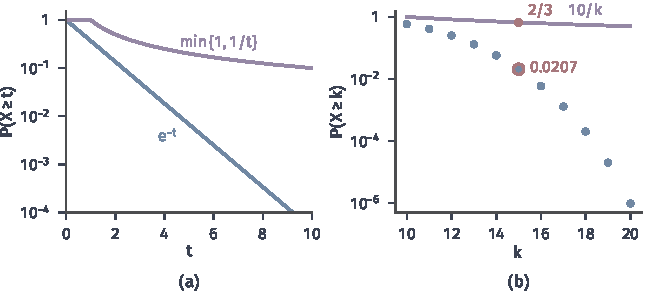
\includegraphics[width=112mm]{figures/07-probability/01-elementary-probability/matplotlib/tail-markov-compare/figure.pdf}
 \caption{Markov界（紫线）与精确尾概率（蓝色），纵轴为对数刻度。(a)$X\sim\operatorname{Exp}(1)$，精确值$\mathrm{e}^{-t}$。(b)$X\sim\operatorname{Bin}(20,1/2)$，蓝点为$\mathbb{P}(X\geq k)$，紫线为$10/k$，红色标出$k=15$处的$2/3$与$0.0207$。}
 \label{fig:tail-markov-compare}
\end{BookInlineFigure}

\paragraph{一般形式}
压住示性函数的不必是直线。只要函数$g$非负且不减，事件$\{X\geq t\}$就包含在$\{g(X)\geq g(t)\}$之中，对$g(X)$用Markov不等式即可。下面的形式是后面三节的共同出发点。

\begin{lemma}[Markov不等式的一般形式]
\label{lem:tail-markov-general}
设$g$是$\mathbb{R}$上的非负不减函数，$t$满足$g(t)>0$，且$\mathbb{E}[g(X)]<\infty$。则
\begin{equation}
 \mathbb{P}(X\geq t)\leq\frac{\mathbb{E}[g(X)]}{g(t)} .
 \label{eq:tail-markov-general}
\end{equation}
\end{lemma}

\begin{proof}
若$X\geq t$，由$g$不减得$g(X)\geq g(t)$，所以$\{X\geq t\}\subseteq\{g(X)\geq g(t)\}$，前者的概率不超过后者。$g(X)$非负，期望有限，$g(t)>0$，对它用定理~\ref{thm:tail-markov}：
\[
 \mathbb{P}(X\geq t)\leq\mathbb{P}\bigl(g(X)\geq g(t)\bigr)\leq\frac{\mathbb{E}[g(X)]}{g(t)} .
\]
这就是式~\eqref{eq:tail-markov-general}。
\end{proof}

这里不再要求$X\geq0$，非负性转移给了$g$。选择$g$就是选择要用分布的哪一项信息：对非负变量$\lvert X-a\rvert$取$g(s)=\max\{s,0\}^p$，用的是$p$阶绝对矩；对$X$本身取$g(x)=\mathrm{e}^{\lambda x}$，用的是指数矩。$g$在远处增长越快，远处的质量在$\mathbb{E}[g(X)]$里被放得越大，界就可能衰减得越快；代价是$\mathbb{E}[g(X)]$有限的要求越强。
